\documentclass{article}
\usepackage{lmodern}
\usepackage[T1]{fontenc}
\usepackage{shapepar}
\usepackage{microtype}
\usepackage{lipsum}
\usepackage{pgfplots}
\pgfplotsset{compat=1.9}
\usepackage{tikz}
\usetikzlibrary{calc,fit,intersections,folding}
\usepackage{pstricks-add}
\usetikzlibrary{arrows.meta,angles,arrows,quotes,backgrounds}

\newcommand{\tubecolor}{red}
\newcommand{\thickness}{0.5mm}
\newcommand{\n}{2mm}


\begin{document}
\thispagestyle{empty}
\begin{center}
    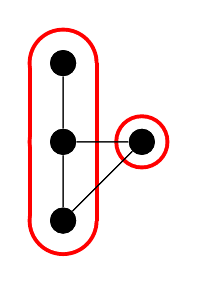
\begin{tikzpicture}
        \begin{scope}
        \node[fill] (A) at (0,0) [circle] {};
        \node[fill] (B) at (0,-1) [circle] {};
        \node[fill] (C) at (0,-2) [circle] {};
        \node[fill] (D) at (1,-1) [circle] {};
    
        \draw (A) -- (B) -- (C) -- (D) (B) -- (D);
        \node[fill] (A) at (0,0) [circle] {};
        \node[fill] (B) at (0,-1) [circle] {};
        \node[fill] (C) at (0,-2) [circle] {};
        \node[fill] (D) at (1,-1) [circle] {};
    
        \draw (A) -- (B) -- (C) -- (D) (B) -- (D);
        %Tube ABC:
        \begin{scope}[on background layer]
            \fill[\tubecolor] (B) circle (\n + 5*\thickness);
            \fill[\tubecolor] (A) circle (\n + 5*\thickness);
            \fill[\tubecolor] (C) circle (\n + 5*\thickness);
            \draw[\tubecolor] [line width = 2*(\n + 5*\thickness)] (A.center) -- (C.center);
            
            \fill[white] (B) circle (\n + 4*\thickness);
            \fill[white] (A) circle (\n + 4*\thickness);
            \fill[white] (C) circle (\n + 4*\thickness);
            \draw[white] [line width = 2*(\n + 4*\thickness)] (A.center) -- (C.center);
        \end{scope}
        %Tube D:
        \begin{scope}[on background layer]
            \fill[\tubecolor] (D) circle (\n + 3*\thickness);
            
            \fill[white] (D) circle (\n + 2*\thickness);
        \end{scope}
    \end{scope}
    \end{tikzpicture}
    \end{center}
    \end{document}